\subsection{Sombras}
Los resultados obtenidos en la \autoref{fig:difBlinn} presentan ciertas carencias, siendo la más flagrante la ausencia de sombras arrojadas, que no son consideradas en el modelo de Blinn-Phong. Afortunadamente el uso de las SDFs nos hará la obtención de la información necesaria para añadir sombras a nuestra escena muy sencilla. Para saber si un punto $p\in\R^3$ recibe luz de una $i$-ésima fuente de luz bastará comprobar si hay algún obstáculo entre dicha fuente y el punto. Para hacer esta comprobación usaremos de nuevo \textit{spheretracing}, pero en esta ocasión desde el punto hacia la fuente de luz. Si se detecta alguna intersección significará que el punto $p$ no recibe luz de la fuente y por tanto $L_R(p,v,l_i) = 0,\ \forall v\in \R^3$. Podemos modificar \texttt{DibujarSuperficie} como se muestra en la \autoref{fig:sombras1} para añadir este comprobación.\newline

\begin{algorithm}[H]
        \caption{DibujarSupercicie}
            \KwData{punto $p$, dirección del rayo $v$, distancia $\phi(p)$}
            \KwResult{terna RGB con la radiancia percibida en el punto $p$}
            $L \gets L_A + L_E$ \Comment{Radiancia final}
            \For{$i \in \{1,\dots, n\}$} {

                \Comment{ ··· }
                $sombras \gets CalcularSombras(p, l_i)$

                $L \gets L + S_i\cdot (f_{ra} + f_{rd} + f_{re})\cdot sombras$
            }

            \Return{$L$}
    \end{algorithm}
\begin{figure}[ht!]
    \centering
    \begin{minipage}{0.50\textwidth}
   \begin{algorithm}[H]
            \caption{CalcularSombras}
                \KwData{punto $p_0$, dirección de luz $l_i$}
                \KwResult{factor de sombra en $p_0$ en el rango $[0,1]$}
                 $d \gets \delta$ \Comment{distancia actual}
                
                \For{i $\in$ MAX\_ITERACIONES} {
                    $p \gets p_o + d \cdot v$
                    
                    $sdf \gets \phi(p)$
                    
                    \If{sdf $< \varepsilon$}{
                       \Return{0};
                    }
            
                    $d \gets d + sdf$

                    \If{d > MAX\_DISTANCIA}{
                        \Return{1}
                    }
                }

                \Return{1}
        \end{algorithm}
    \end{minipage}%
    \hfill
    \begin{minipage}{0.48\textwidth}
        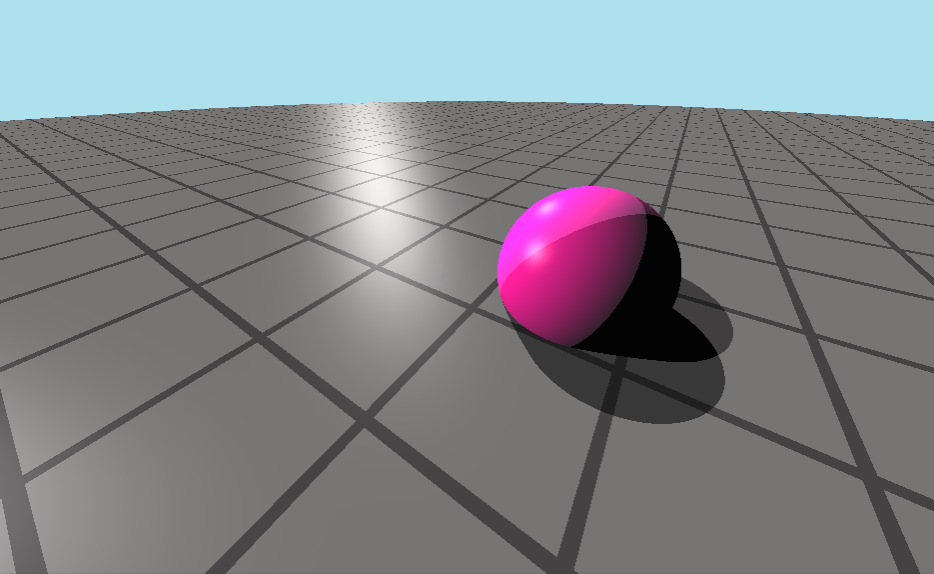
\includegraphics[width=\textwidth]{shadowSimple.png}
    \end{minipage}
    \caption{Cálculo básico de sombras}
    \label{fig:sombras1}
\end{figure}


Realizamos las siguientes apreciaciones respecto al método \texttt{CalcularSombras} propuesto:
\begin{itemize}
    \item Dado que estamos trabajando con luces direccionales situadas a distancia infinita solo podemos hacer \textit{spheretracing} desde $p$ en dirección a la fuente, a pesar de que lo intuitivo sería hacerlo desde el foco de luz hacia el punto.
    \item A diferencia del algoritmo propuesto en \autoref{a:spheretracing} no podemos inicializar $d=0$, ya que entonces se detectaría una intersección en el mismo punto $p$.
\end{itemize}

Estudiando los resultados obtenidos vemos que al añadir sombras obtenemos una imagen mucho más cohesiva y otorgamos a la esfera mayor presencia en la escena. Sin embargo también podremos apreciar que las sombras que genera este método son muy planas y duras. Realmente ahora mismo no tenemos control alguno sobre esto, ya que según nuestra implementación un punto o está totalmente en sombra o totalmente iluminado. Esto no siempre es así en el mundo real, donde podemos encontrar que no toda la región sombreada sea igual de oscura o el borde esté más o menos difuminado en función de las propiedades de la fuente. Podemos simular estos fenómenos de forma muy sencilla usando información de la que ya que disponemos en el algoritmo de \textit{spheretracing}. En particular:
\begin{itemize}
    \item Haremos que cuanto más cerca se encuentre el punto del obstáculo que le hace sombra menos luz reciba. Por tanto la intensidad de la sombra será proporcional a la evaluación de la SDF en el punto actual del rayo:
    \begin{equation*}
        sombra \propto sdf.
    \end{equation*}
    \item Cuando un punto sea alcanzado por la luz pero haya estado muy cerca de ser obstruido dejaremos que refleje solo una fracción de la luz total. Esta cantidad deberá ser mayor cuanto menos haya faltado para perder la intersección, creando un difuminado en el borde:
    \begin{equation*}
        sombra \propto \frac{1}{d}.
    \end{equation*}
\end{itemize}

Esta nueva versión de \texttt{CalcularSombras} se encuentra descrita en la \autoref{fig:sombras2}. En ella se ha añadido un parámetro $k\in \R_0^+$ para controlar la intensidad del efecto de suavizado. En realidad este parámetro hace referencia al \textbf{tamaño de la fuente de luz}, en concreto a su inversa. Así, cuanto más pequeño sea este valor más grande será la fuente de luz, produciendo sombras más difusas. Por ejemplo, el Sol tendrá un valor pequeño para $k$, mientras que una bombilla lo tendría grande. A partir de ahora en nuestra escena de ejemplo fijamos $k=  1.5$ para la fuente de luz que apunta más hacia la cámara, que actuará como el Sol, y $k = 10$ para la otra, que actuará como una linterna.\newline

\begin{figure}[ht!]
    \centering
    \begin{minipage}{0.50\textwidth}
       \begin{algorithm}[H]
            \caption{CalcularSombras}
                \KwData{punto $p_0$, dirección de luz $l_i$, tamaño de luz $k$}
                \KwResult{factor de sombra en $p_0$ en el rango $[0,1]$}
                $sombra \gets 1$
                
                $d \gets \delta$ \Comment{distancia actual}
                
                \For{i $\in$ MAX\_ITERACIONES} {
                    $p \gets p_o + d \cdot v$
                    
                    $sdf \gets \phi(p)$
                    
                    \If{sdf $< \varepsilon$}{
                       \Return{0};
                    }
                    $sombra \gets \Min(sombra, k\cdot \frac{sdf}{d})$
                    
                    $d \gets d + sdf$

                    \If{d > MAX\_DISTANCIA}{
                        \Return{1}
                    }
                }

                \Return{1}
        \end{algorithm}
    \end{minipage}%
    \hfill
    \begin{minipage}{0.48\textwidth}
        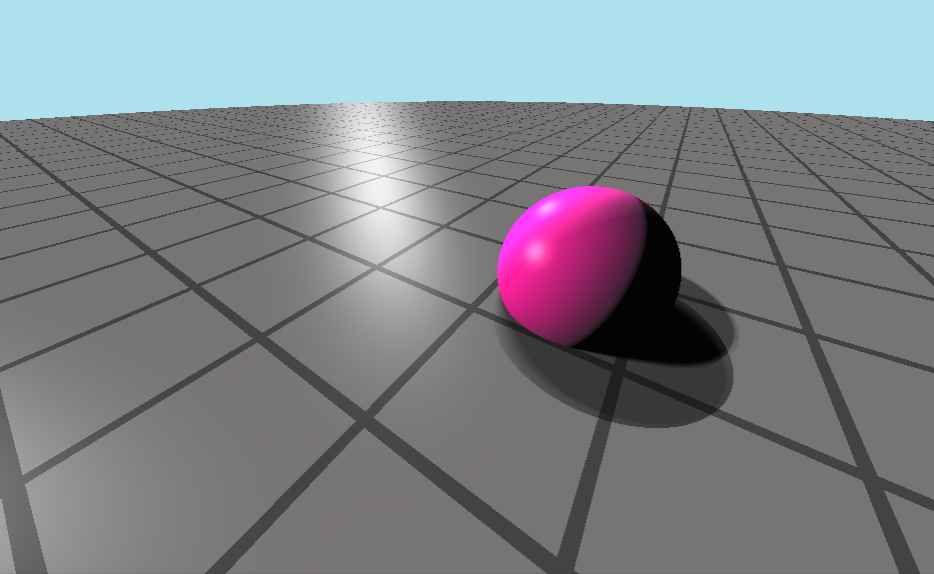
\includegraphics[width=\textwidth]{shadowSoftArtifact.png}
    \end{minipage}
    \caption{Cálculo de sombras suavizadas}
    \label{fig:sombras2}
\end{figure}

Si bien este método genera resultados más realistas en general, también puede generar ciertas imperfecciones en el borde de la sombra, como se puede apreciar en la \autoref{fig:artifactZoom}. Esto es debido a que en el proceso de \textit{spheretracing} podemos saltarnos una intersección que habría aportado más oscuridad que la que finalmente se ha encontrado, generando fugas de luz que siguen el patrón de los puntos en los que se evalúa la SDF. Hay varias formas de solventar esto, como la propuesta por Sebastian Aaltonen \cite{gdc} en la GDC de 2018. Su idea se basa en comprobar intersecciones también en los puntos que se estiman como los más cercanos a la superficie en cada iteración. Nosotros usaremos una técnica introducida por el usuario \texttt{nurof3n} \cite{shadertoy-sombras} en Shadertoy y estudiada posteriormente por Íñigo Quílez.\newline

\begin{figure}[ht!]
    \centering
    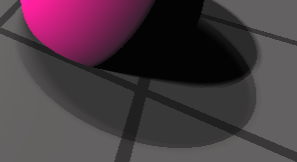
\includegraphics[width=0.7\textwidth]{Plantilla-TFG-master/img/shadowArtifactZoom.png}
    \caption{Detalle de las fugas de luz al calcular sombras}
    \label{fig:artifactZoom}
\end{figure}

La diferencia con nuestro método actual radica en que se permite que el rayo penetre un poco la superficie para detectar los puntos que casi no son alcanzados por un rayo de luz. Por tanto, ahora para cada punto se tiene en cuenta si casi ha sido alcanzado y si casi no ha sido alcanzado por un rayo de luz. Para permitir que el rayo entre en la geometría basta con modificar la condición de ruptura sobre $sdf$ a un número negativo, con la precaución de siempre sumar una cantidad positiva a $d$, pues de lo contrario el trazado del rayo retrocedería. Fijando este valor a $-1$ la variable $sombra$ tendrá un valor en el rango $[-1,1]$ al salir del bucle, pero aún queremos obtener un valor entre $[0,1]$ para representar la cantidad de luz que recibe el punto. Para remapear $sombra$ a este rango podemos usar la función \texttt{smoothstep(a,b,x)} de GLSL, que interpola $x$ suavemente entre $0$ y $1$ en relación con los límites $a$ y $b$. En particular la interpolación que se lleva a cabo es la de Hermite, haciendo que la transición entre distintos puntos de sombra no sea lineal y parezca más natural. Podemos ver el algoritmo final en la \autoref{fig:sombras3} y los resultados que consigue en la \autoref{fig:sombras4}.

\begin{figure}[ht!]
    \centering
    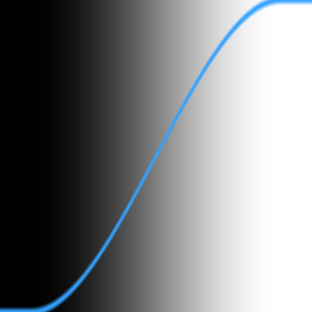
\includegraphics[width=0.3\textwidth]{Plantilla-TFG-master/img/smoothstep.png}
    \caption{Visualización de \texttt{smoothstep} \cite{smoothstep}}
    \label{fig:miss}
\end{figure}

\begin{figure}[ht!]
    \centering
   \begin{algorithm}[H]
        \caption{CalcularSombras}
            \KwData{punto $p_0$, dirección de luz $l_i$, tamaño de luz $k$}
            \KwResult{valor en el rango $[0,1]$ representando la cantidad de sombra recibida en $p_0$}
            $sombra \gets 1$
            
            $d \gets \delta$ \Comment{distancia actual}
            
            \For{i $\in$ MAX\_ITERACIONES} {
                $p \gets p_o + d \cdot v$
                
                $sombra \gets \Min(res, k\cdot \frac{sdf}{d})$
                
                $sdf \gets \phi(p)$

                $d \gets d + \vert sdf\vert$
                
                \If{$sombra < -1 $ \textbf{OR} $d > MAX\_DISTANCIA$}{
                   \textbf{break}
                } 
            }

            \Return{$smoothstep(-1,1,sombra)$}
    \end{algorithm}

    \caption{Cálculo de sombras suavizadas mejorado}
    \label{fig:sombras3}
\end{figure}

\begin{figure}[ht!]
    \centering
    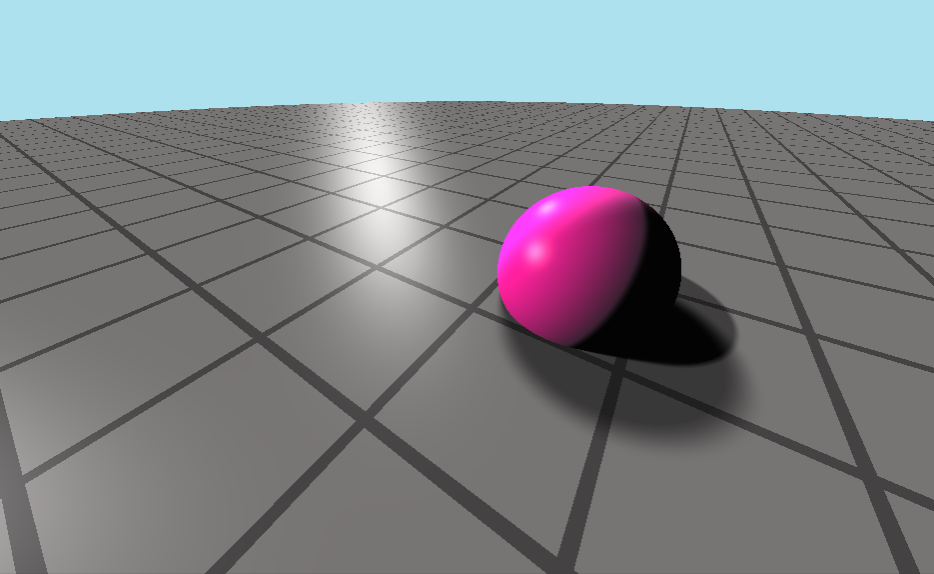
\includegraphics[width=\textwidth]{Plantilla-TFG-master/img/shadowSoft.png}
    \caption{Resultado final del cálculo de sombras}
    \label{fig:sombras4}
\end{figure}


